\documentclass[../Main.tex]{subfiles}

\begin{document}

\section{Design und Umsetzung des Kampfabschnitts} \label{sec:Umsetzung}

In diesem Kapitel stellen wir zunächst Designvorschläge für die beiden inhaltlichen Komponenten der Erkenntnisfrage (Abschnitt~\ref{sec:Erkenntnisfrage}) auf: Gegnerverhalten einerseits, Gegnerplatzierung und Leveldesign andererseits. Sie zielen auf die drei dort genannten spielerischen Qualitäten ab, nämlich einen nachvollziehbaren Spielfluss, eine angemessene Schwierigkeit und ein befriedigendes Spielgefühl. Dazu verdichten wir die Erkenntnisse aus der Referenzspielanalyse (Abschnitt~\ref{sec:Vergleich}), die vor allem das Gegnerverhalten betreffen, und aus der Leveldesign-Recherche (Abschnitt~\ref{sec:ZwischenfazitLD}), die vor allem die Gegnerplatzierung betreffen, zu spezifischen Designvorschlägen für unseren Kampfabschnitt. Nicht alle Punkte aus der Recherche konnten wir dabei berücksichtigen, da dies im vorgegebenen Zeitraum nicht möglich war. Deshalb haben wir jene Punkte ausgewählt, die wir als besonders wichtig für unsere Erkenntnisfrage oder als im Prototyp überprüfbar eingeschätzt haben.

Für jeden Vorschlag beschreiben wir anschliessend, wie er im Prototyp umgesetzt wurde. Die genaue technische Umsetzung lässt sich im Quellcode des Prototyps nachvollziehen.\footnote{\textcolor{red}{[GitHub-Link einfügen]}} Zur Orientierung im Quellcode stellen wir die technische Dokumentation bereit.\footnote{\textcolor{red}{[Titel der technischen Dokumentation einfügen]}} Wie wir bei der Umsetzung allgemein vorgegangen sind und welche Software wir verwendet haben, beschreibt Abschnitt~\ref{sec:VorgehenUmsetzung}. Ob die Vorschläge die gewünschte Wirkung haben, überprüfen wir in den Playtests (Kapitel~\ref{sec:Evaluation}); sie sind zugleich der Massstab, an dem wir die drei spielerischen Qualitäten messen.

\begin{itemize}[leftmargin=1.5cm]
    \item \textcolor{red}{\enquote{da dies im vorgegebenen Zeitraum nicht möglich war}: Zeitmangel als Grund ist ehrlich, gehört aber eher in die Limitationen (Abschnitt~\ref{sec:Limitationen}). Hier reicht das Auswahlkriterium (wichtig für die Erkenntnisfrage, im Prototyp prüfbar).}
\end{itemize}

\subsection{Von der Recherche zu den Designvorschlägen} \label{sec:Designvorschlaege}

In diesem Abschnitt listen wir die ausgewählten Designvorschläge übersichtlich auf. Wir nennen hier nur ihre Namen und zeigen, aus welchem Teil unserer Recherche sie stammen; in den folgenden Abschnitten wird jeder Vorschlag genau aufgeschlüsselt. Dabei folgt jeder Designvorschlag demselben Schema: der Vorschlag selbst, sein Nutzen, also welcher Aspekt der Erkenntnisfrage damit bedient wird, und die Herleitung aus Recherche und Spielanalysen. Die Vorschläge sind mit V1 bis V8 nummeriert; Tabelle~\ref{tab:Designvorschlaege} gibt einen Überblick. Die beiden Herleitungsspalten zeigen, dass die Vorschläge zum Gegnerverhalten vor allem aus der Referenzspielanalyse stammen und jene zur Gegnerplatzierung zusätzlich auf der Leveldesign-Recherche beruhen.

\begin{table}[H]
    \centering
    \small
    \renewcommand{\arraystretch}{1.3}
    \begin{tabular}{|>{\raggedright\arraybackslash}p{0.6cm}|>{\raggedright\arraybackslash}p{3.4cm}|>{\raggedright\arraybackslash}p{5.2cm}|>{\raggedright\arraybackslash}p{4.3cm}|}
        \hline
        \textbf{Nr.} & \textbf{Designvorschlag} & \textbf{Herleitung aus der Referenzspielanalyse (Kap.~\ref{sec:Referenzspielanalyse})} & \textbf{Herleitung aus der Leveldesign-Recherche (Kap.~\ref{sec:Leveldesign})} \\
        \hline
        \multicolumn{4}{|l|}{\textit{Gegnerverhalten (Abschnitt~\ref{sec:UmsetzungGegner})}} \\
        \hline
        V1 & Überlegenheit als Grundzustand & Kontrast dauerhafte Überlegenheit in \game{NieR: Automata} und prekäre Kontrolle in \game{Ninja Gaiden} (A1 beider Analysen); nicht unterbrechbarer Gegner als Vorbild aus \game{Ninja Gaiden} & Vom gewünschten Gefühl ausgehen (Abschnitt~\ref{sec:Pacing}) \\
        \hline
        V2 & Begrenzung gleichzeitig aktiver Gegner & Gemeinsamkeit beider Spiele: \game{Ninja Gaiden} D1, \game{NieR: Automata} M2 (Abschnitt~\ref{sec:Vergleich}) & -- \\
        \hline
        V3 & Taktisches Dilemma durch Nah- und Fernkämpfer & D2 beider Analysen; in \game{NieR: Automata} versperren Nahkämpfer den Weg zu den Fernkämpfern & -- \\
        \hline
        V4 & Klar telegrafierte Angriffe & \game{NieR: Automata}, M2 & -- \\
        \hline
        \multicolumn{4}{|l|}{\textit{Gegnerplatzierung und Kampfraum (Abschnitt~\ref{sec:UmsetzungLevel})}} \\
        \hline
        V5 & Lesbare Platzierung, dynamisches Verhalten & Symmetrische Anfangsaufstellung in \game{NieR: Automata} (A3); dynamisches Verhalten in \game{Ninja Gaiden} (D3, M2) & Lesbarkeit; \textit{Shrinking Fortress} (Abschnitt~\ref{sec:Encounter}) \\
        \hline
        V6 & Der Raum als Druckmittel & Gezielte Verengung in \game{Ninja Gaiden} (M3) & Raumtypen nach Totten und Rogers (Abschnitt~\ref{sec:Raumtypologien}) \\
        \hline
        V7 & Wellenstruktur mit Erholungsphasen & Wellen mit Nachrücken in \game{Ninja Gaiden} (D1); Arenen und Zwischenpassagen in \game{NieR: Automata} (A4) & Rollercoaster-Pacing (Abschnitt~\ref{sec:Pacing}) \\
        \hline
        V8 & Gestaffelte Einführung neuer Gegner & Aufbau des Prologs in \game{NieR: Automata} (D1) & Scaffolding und Braiding (Abschnitt~\ref{sec:Scaffolding}) \\
        \hline
    \end{tabular}
    \caption{Übersicht der Designvorschläge und ihrer Herleitung}
    \label{tab:Designvorschlaege}
\end{table}

\subsection{Der Prototyp im Überblick} \label{sec:Prototyp}

Unser Prototyp ist ein 3D-Hack-and-Slash-Spiel in der Third-Person-Perspektive, das wir mit der Game Engine Godot entwickelt haben. Es handelt sich um den Prototyp eines einzelnen, zusammenhängenden Kampfabschnitts aus zwölf Räumen und nicht um ein vollständiges Spiel. Bevor wir in den Abschnitten~\ref{sec:UmsetzungGegner} und~\ref{sec:UmsetzungLevel} die Umsetzung der einzelnen Designvorschläge beschreiben, stellen wir hier die Spielfigur, die fünf Gegnertypen (Abschnitt~\ref{sec:Gegnertypen}) sowie den Aufbau des Kampfabschnitts und das Wellensystem (Abschnitt~\ref{sec:Kampfabschnitt}) vor.

\subsubsection{Spieler und Gegnertypen} \label{sec:Gegnertypen}

\paragraph{Spielfigur}
Zuerst stellen wir die Spielfigur vor, die von den Spielern gesteuert wird. Sie kann sich frei in alle Richtungen bewegen und springen. Der Sprung ist adaptiv: Je länger man die Taste gedrückt hält, desto höher springt die Figur. Zusätzlich verfügt sie über zwei Doppelsprünge, kann also insgesamt dreimal hintereinander springen. Ausserdem kann sie dashen; hält man die Dash-Taste gedrückt, rennt sie mit erhöhter Geschwindigkeit weiter. Beim Hochspringen kann sie sich zudem an Kanten festhalten (\textit{Ledge Grab}).

Die Spielfigur hat eine grüne Lebensleiste mit 200 Lebenspunkten und eine blaue Energieleiste, die sich füllt, wenn sie Gegner trifft. Mit dieser Energie kann sie sich heilen: Jede Heilung stellt 50 Lebenspunkte wieder her, eine volle Energieleiste reicht also für genau 200 Lebenspunkte und damit für eine vollständige Heilung. Das Heilen dauert eine gewisse Zeit, in der sich die Spielfigur nicht bewegen kann. Der Spieler kann das Heilen nicht selbst abbrechen; wird die Spielfigur währenddessen getroffen, bricht es jedoch ab.

Angreifen kann die Spielfigur mit einem leichten und einem schweren Angriff (\textit{Light Attack} und \textit{Heavy Attack}). Aus diesen beiden Eingaben ergeben sich sechs Combos, die Tabelle~\ref{tab:Combos} zeigt.

\begin{table}[H]
    \centering
    \small
    \renewcommand{\arraystretch}{1.5}
    \begin{tabular}{|l|l|l|r|}
        \hline
        \textbf{Combo} & \textbf{Eingabe} & \textbf{Schaden pro Treffer} & \textbf{Gesamt} \\
        \hline
        Light Combo & \fbox{\textsf{L}}\,$\rightarrow$\,\fbox{\textsf{L}}\,$\rightarrow$\,\fbox{\textsf{L}}\,$\rightarrow$\,\fbox{\textsf{L}} & 20, 20, 30, 40 & 110 \\
        \hline
        Light-Variante 1 & \fbox{\textsf{L}}\,$\rightarrow$\,\fbox{\textsf{P}}\,$\rightarrow$\,\fbox{\textsf{L}}\,$\rightarrow$\,\fbox{\textsf{L}} & 20, 30, 40 & 90 \\
        \hline
        Light-Variante 2 & \fbox{\textsf{L}}\,$\rightarrow$\,\fbox{\textsf{L}}\,$\rightarrow$\,\fbox{\textsf{P}}\,$\rightarrow$\,\fbox{\textsf{L}} & 20, 20, 40 & 80 \\
        \hline
        Heavy Combo & \fbox{\textsf{H}}\,$\rightarrow$\,\fbox{\textsf{H}}\,$\rightarrow$\,\fbox{\textsf{H}} & 30, 30, 40 & 100 \\
        \hline
        Gemischte Combo & \fbox{\textsf{H}}\,$\rightarrow$\,\fbox{\textsf{L}}\,$\rightarrow$\,\fbox{\textsf{L}}\,$\rightarrow$\,\fbox{\textsf{L}}\,$\rightarrow$\,\fbox{\textsf{L}} & 30, 30, 20, 30, 40 & 150 \\
        \hline
        Air Combo & \fbox{\textsf{L}}\,$\rightarrow$\,\fbox{\textsf{L}}\,$\rightarrow$\,\fbox{\textsf{L}}\,$\rightarrow$\,\fbox{\textsf{L}} (in der Luft) & 20, 20, 20, 20 & 80 \\
        \hline
    \end{tabular}
    \caption{Combos des Spielers mit Eingabe und Schaden (\textsf{L} = leichter Angriff, \textsf{H} = schwerer Angriff, \textsf{P} = kurze Pause)}
    \label{tab:Combos}
\end{table}

\begin{itemize}[leftmargin=1.5cm]
    \item \textcolor{red}{Wie lange dauert das Heilen ungefähr (Sekunden)? Ein Wert macht die Aussagen in V1 (\enquote{Das Heilen dauert eine gewisse Zeit}) und in Kapitel~\ref{sec:Evaluation} (TP2 wurde beim Heilen unterbrochen) nachvollziehbar.}
\end{itemize}

\paragraph{Gegnertypen}
In unserem Prototyp gibt es zwei Gegnerklassen, Nah- und Fernkämpfer, von denen es jeweils mehrere Varianten gibt: zwei Nahkämpfer und drei Fernkämpfer. Insgesamt gibt es damit fünf verschiedene Gegnertypen (Abbildung~\ref{fig:Gegnertypen}). Farblich sind die Nahkämpfer in Rottönen und die Fernkämpfer in Gelb- bis Orangetönen gehalten. Die Einteilung in Nah- und Fernkämpfer mit leichteren und schwereren Varianten übernehmen wir aus den beiden Referenzspielen (Frage~M1 beider Analysen, Abschnitt~\ref{sec:Vergleich}); Heavy Archer und Chain Archer sind dagegen unsere eigene Erweiterung.

\begin{figure}[H]
    \centering
    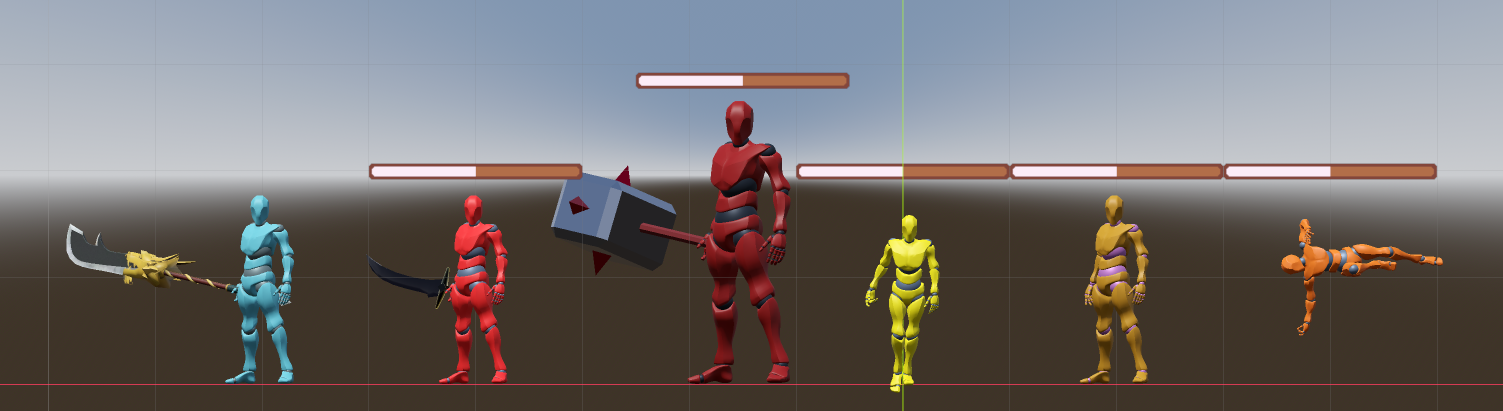
\includegraphics[width =\linewidth]{Assets/All Entities.png}
    \caption[Die fünf Gegnertypen des Prototyps. Eigene Abbildung.]{Die fünf Gegnertypen des Prototyps und der Spieler, von links nach rechts: Spieler (Blau), Soldier (Rot), Heavy Soldier (Dunkelrot), Archer (Gelb), Heavy Archer (Hellbraun), Chain Archer (Orange). Eigene Abbildung.}
    \label{fig:Gegnertypen}
\end{figure}

Der Soldier ist der grundlegende Nahkämpfer, der auf den Spieler zurennt und zuschlägt. Der Heavy Soldier ist grösser, stärker und langsamer als der Soldier und hat mehr Lebenspunkte, zeigt aber dasselbe Verhalten. Als einziger Gegner lässt er sich nicht unterbrechen. Damit setzen wir die Erkenntnis aus Abschnitt~\ref{sec:Vergleich} um, die Überlegenheit des Spielers wie in \game{Ninja Gaiden} gezielt durch einen Gegner zu brechen, der sich nicht unterbrechen lässt (Abschnitt~\ref{sec:V1}).

Die Fernkämpfer bewegen sich alle nicht. Der Archer schiesst ein Projektil auf den Spieler. Der Heavy Archer macht dasselbe, sein Projektil ist jedoch langsamer, kann dafür die Richtung ändern und verfolgt den Spieler. Der Chain Archer schiesst gleich drei Pfeile auf den Spieler, die mehr als doppelt so schnell sind wie jene des Archers.

Die Reichweite der Archers, also die Distanz, aus der sie auf den Spieler schiessen können, ist bei allen drei Typen gleich. Lebenspunkte und Schaden unterscheiden sich dagegen je nach Gegnertyp; Tabelle~\ref{tab:Gegnertypen} fasst die Eigenschaften zusammen.

\begin{table}[H]
    \centering
    \small
    \renewcommand{\arraystretch}{1.3}
    \begin{tabular}{|>{\raggedright\arraybackslash}p{2.3cm}|>{\raggedright\arraybackslash}p{2.9cm}|>{\raggedright\arraybackslash}p{3.0cm}|>{\raggedright\arraybackslash}p{0.8cm}|>{\raggedright\arraybackslash}p{1.4cm}|>{\raggedright\arraybackslash}p{1.9cm}|}
        \hline
        \textbf{Gegnertyp} & \textbf{Bewegung} & \textbf{Angriff} & \textbf{LP} & \textbf{Schaden} & \textbf{Unter\-brechbar} \\
        \hline
        \multicolumn{6}{|l|}{\textit{Nahkämpfer (Rottöne)}} \\
        \hline
        Soldier & rennt auf den Spieler zu & Nahkampfschlag & 130 & 15 & ja \\
        \hline
        Heavy Soldier & wie Soldier, aber langsamer; grösser & wie Soldier & 200 & 30 & nein \\
        \hline
        \multicolumn{6}{|l|}{\textit{Fernkämpfer (Gelb- bis Orangetöne)}} \\
        \hline
        Archer & stationär & ein Projektil & 60 & 10 & ja \\
        \hline
        Heavy Archer & stationär & ein langsameres, zielsuchendes Projektil & 40 & 20 & ja \\
        \hline
        Chain Archer & stationär & drei Pfeile, mehr als doppelt so schnell wie beim Archer & 70 & $3 \times 10$ & ja \\
        \hline
    \end{tabular}
    \caption{Eigenschaften der fünf Gegnertypen (LP = Lebenspunkte)}
    \label{tab:Gegnertypen}
\end{table}

\paragraph{Abstimmung von Schaden und Lebenspunkten}
Der Spieler hat 200 Lebenspunkte, seine Angriffe verursachen je nach Combo unterschiedlich viel Schaden (Tabelle~\ref{tab:Combos}).

Die Schadenswerte und Lebenspunkte wurden so gewählt, dass bestimmte Combos einen Gegner genau mit dem letzten Schlag besiegen, weil wir davon ausgingen, dass sich dies besser anfühlt: Eine Heavy Combo besiegt einen Chain Archer mit ihrem letzten Schlag, und der Heavy Soldier stirbt nach genau zwei Heavy Combos. Gleichzeitig haben wir darauf geachtet, dass zum Beispiel ein Soldier eine Light Combo knapp überlebt. Dadurch entsteht beim Spielen Variation, und der Spieler muss Combos abbrechen oder kombinieren.

\begin{itemize}[leftmargin=1.5cm]
    \item \textcolor{red}{\enquote{weil wir davon ausgingen, dass sich dies besser anfühlt}: ist als eure Annahme gekennzeichnet, gut. In Kapitel~\ref{sec:Evaluation} aufgreifen, falls die Testpersonen etwas dazu gesagt haben.}
    \item \textcolor{red}{Gemeinsame Basisklasse der Gegner: nur mit Verweis auf die technische Dokumentation nennen. Der frühere Rückbezug auf Abschnitt~4.1 (Kernmechanik) entfällt, wenn 4.1 gestrichen wird.}
\end{itemize}

\subsubsection{Kampfabschnitt und Wellensystem} \label{sec:Kampfabschnitt}

Unser Kampfabschnitt besteht aus zwölf Encountern, also zwölf abgeschlossenen Kämpfen. Jeder Encounter findet in einem Raum statt und besteht aus mehreren Wellen; Anzahl und Grösse der Wellen sind für jeden Encounter speziell konfiguriert. Da Encounter~3 und Encounter~12 im selben Raum stattfinden, verteilen sich die zwölf Encounter auf elf Räume. Wenn wir im Folgenden von einem Raum mit Nummer sprechen (z.\,B.\ Raum~6), meinen wir den Raum, in dem der Encounter mit dieser Nummer stattfindet. Eine neue Welle erscheint erst, nachdem alle Gegner der vorherigen Welle besiegt wurden. Eine Welle enthält zwischen 1 und 20 Gegner.

Der Kampfabschnitt beginnt bei Encounter~1 und endet bei Encounter~12. Wie Abbildung~\ref{fig:Map} zeigt, ist er als Rundgang aufgebaut, sodass der Spieler am Ende in den Raum von Encounter~3 zurückkehrt. Der Raum von Encounter~11 liegt direkt darüber; am Ende von Encounter~11 springt der Spieler hinunter in den Raum von Encounter~12.

\begin{figure}[H]
    \centering
    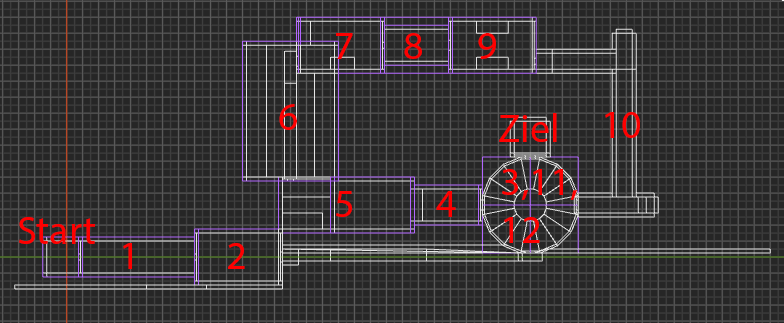
\includegraphics[width=\linewidth]{Assets/Map Layout.png}
    \caption[Grundriss des Kampfabschnitts. Eigene Abbildung.]{Grundriss des Kampfabschnitts mit den Nummern der Encounter, Start und Ziel (Draufsicht aus TrenchBroom). Der Kampfabschnitt ist als Rundgang aufgebaut: Encounter~12 findet im selben Raum statt wie Encounter~3, und der Raum von Encounter~11 liegt gleich gross direkt darüber. Deshalb sind die drei Encounter an derselben Stelle eingezeichnet. Eigene Abbildung.}
    \label{fig:Map}
\end{figure}

Pro Welle lässt sich zudem festlegen, wie viele Gegner gleichzeitig im Raum sein dürfen; in unseren Encountern sind es meist drei bis sechs, im finalen Encounter zur Eskalation bis zu acht (Abschnitt~\ref{sec:V2}). Stirbt ein Gegner, rückt ein weiterer nach, wie wir es auch in \game{Ninja Gaiden} beobachtet haben (Abschnitt~\ref{sec:ReferenzspielanalyseNinja}, Frage~D1). Die Reihenfolge, in der die Gegner erscheinen, ist im Voraus festgelegt. Jede Welle besteht aus einem Teil fest platzierter und einem Teil zufällig erscheinender Gegner (Abschnitt~\ref{sec:V5}). Nachdem alle Wellen eines Encounters besiegt wurden, öffnet sich genau eine Tür, durch die der Spieler weitergehen kann.

Tabelle~\ref{tab:Raeume} zeigt den Aufbau der einzelnen Encounter und den Typ des Raumes, in dem sie stattfinden; die Raumtypen werden in Abschnitt~\ref{sec:V6} erläutert.

{\small
    \renewcommand{\arraystretch}{1.3}
    \begin{longtable}{|>{\raggedright\arraybackslash}p{0.9cm}|>{\raggedright\arraybackslash}p{1.6cm}|>{\raggedright\arraybackslash}p{1.1cm}|>{\raggedright\arraybackslash}p{5.5cm}|>{\raggedright\arraybackslash}p{3.6cm}|}
        \hline
        \textbf{Nr.} & \textbf{Raumtyp} & \textbf{Wellen} & \textbf{Ablauf} & \textbf{Funktion} \\
        \hline
        \endfirsthead
        \hline
        \textbf{Nr.} & \textbf{Raumtyp} & \textbf{Wellen} & \textbf{Ablauf} & \textbf{Funktion} \\
        \hline
        \endhead
        \multicolumn{5}{r}{\textit{Fortsetzung auf der nächsten Seite}} \\
        \endfoot
        \caption{Aufbau der Encounter des Kampfabschnitts (Nr. = Nummer des Encounters)}
        \label{tab:Raeume}
        \endlastfoot
        1 & Intimate & 2 & Welle 1: ein Soldier. Welle 2: fünf Soldiers, höchstens zwei gleichzeitig. & Einführung des Soldiers; Spiel erklären \\
        \hline
        2 & Intimate & 2 & Welle 1: ein Archer. Welle 2: fünf Archer, höchstens zwei gleichzeitig. & Einführung des Archers \\
        \hline
        3 & Prospect & 3 & Pro Welle insgesamt etwa 10--15 Gegner, gemischt. & Erstmals gemischte Gegnertypen; Formationen und Dilemma (V3) werden vorgestellt \\
        \hline
        4 & Narrow & 3 & Welle 1: ein einzelner Soldier mit Überraschungsangriff. Welle 2: der Heavy Soldier alleine. Welle 3: Heavy Soldier in Kombination mit dem Archer. & Einführung des Heavy Soldiers; erste Plattform (Box), auf der man sich vor den Gegnern ausruhen kann \\
        \hline
        5 & Prospect & 2 & Welle 1: Archer, Soldier, Heavy Soldier. Welle 2: Archer, Soldier. & Üben des Gelernten; neue Hindernisformation \\
        \hline
        6 & Prospect & 3 & Welle 1: ein Heavy Archer. Welle 2: Heavy Archer zusammen mit Heavy Soldier und Soldier. Welle 3: wie Welle 2. & Einführung des Heavy Archers; Brücke als neues Hindernis \\
        \hline
        7 & Intimate & 3 & Welle 1: Archers und Heavy Archers. Welle 2: ein einzelner Chain Archer. Welle 3: Soldiers und Chain Archers in Kombination. & Einführung des Chain Archers \\
        \hline
        8 & Narrow & 3 & Welle 1: Heavy Soldier, Chain Archer und Heavy Archer gleichzeitig. Wellen 2 und 3: zusätzlich Soldiers und Archers in wechselnden Kombinationen; insgesamt mehr Gegner, aber nicht mehr gleichzeitig. & Der Kampf beginnt nicht beim Betreten, sondern erst, wenn der Spieler den Raum verlassen will \\
        \hline
        9 & Intimate & 2 & Welle 1: alle Gegnertypen ausser dem Archer. Welle 2: alle Gegnertypen ausser dem Soldier. & Alle Gegnertypen sind eingeführt; die Schwierigkeit wird gesteigert \\
        \hline
        10 & Narrow & 3 & Welle 1: Chain Archer und Heavy Archer. Welle 2: Heavy Soldier, Chain Archer und Heavy Archer. Welle 3: Heavy Soldiers und Soldiers sowie ein Heavy Archer. & Einziger Raum, der sich wegen vieler Verzweigungen nicht überblicken lässt \\
        \hline
        11 & Prospect & 1 & Heavy Archer, Heavy Soldier und Heavy Archer, die einzeln nacheinander erscheinen. & Wirkt wie ein Bossraum, enthält aber nur drei Gegner; bewusste Täuschung des Spielers und Ruhe vor dem Sturm vor dem finalen Kampf \\
        \hline
        12 & Prospect & 2 & Welle 1: ein einzelner Archer in der Mitte. Welle 2: Heavy Soldiers, Heavy Archers und Chain Archers sowie Soldiers und Archers. & Finaler Kampf; mehr Gegner als in den übrigen Encountern und gehäuft schwere Gegnertypen \\
        \hline
    \end{longtable}
}

Die meisten Encounter und Wellen führen eine Neuerung ein oder sind so gestaltet, dass sie einen der Designvorschläge unterstützen. Das gilt jedoch nicht für alle: Einige Wellen dienen primär dem Pacing oder dazu, einen Raum etwas länger zu bespielen. Neben den Neuerungen soll schliesslich auch genügend Gelegenheit bleiben, das Gelernte einfach zu spielen. Wir gehen deshalb nicht auf jede einzelne Welle ein. Wo die Konfiguration von Räumen und Gegnern für einen Designvorschlag wichtig ist, erläutern wir unsere Absichten in den folgenden Abschnitten zu den einzelnen Designvorschlägen.

\subsection{Gegnerverhalten und Spieler-Gegner-Interaktion} \label{sec:UmsetzungGegner}

In diesem und dem folgenden Abschnitt beschreiben wir die Umsetzung der acht Designvorschläge. Wir beginnen mit den Vorschlägen zum Gegnerverhalten und zur Spieler-Gegner-Interaktion (V1--V4); anschliessend folgen jene zum Levelaufbau und zur Gegnerplatzierung (V5--V8, Abschnitt~\ref{sec:UmsetzungLevel}).

\subsubsection{V1: Überlegenheit als Grundzustand} \label{sec:V1}

\paragraph{Vorschlag und Herleitung}
Der Spieler soll sich seinen Gegnern grundsätzlich überlegen fühlen, wobei dieser Zustand gezielt durchbrochen werden kann. Der Nutzen liegt im Spielgefühl: Aggression soll sich sicher und belohnt anfühlen, während Spannung erst dort entsteht, wo die Kontrolle kurzzeitig bedroht wird. Hergeleitet ist der Vorschlag aus dem Kontrast der beiden Referenzspiele, der dauerhaften Überlegenheit in \game{NieR: Automata} (Abschnitt~\ref{sec:ReferenzspielanalyseNier}) gegenüber dem prekären Gleichgewicht in \game{Ninja Gaiden} (Abschnitt~\ref{sec:ReferenzspielanalyseNinja}), sowie aus dem Prinzip des emotionsgeleiteten Designs (Abschnitt~\ref{sec:Pacing}).

\paragraph{Umsetzung im Prototyp}
Im Eins-gegen-eins ist der Spieler jedem einzelnen Gegner deutlich überlegen. Er hat je nach Gegnertyp etwa 1,5- bis 5-mal so viele Lebenspunkte wie ein einzelner Gegner, mit Ausnahme des Heavy Soldiers, der mit 200 Lebenspunkten genau gleich viele hat. Auch pro Treffer verursacht der Spieler mit 20 bis 40 Schaden meist mehr als die Gegner mit 10 bis 20 Schaden pro Schlag bzw.\ Pfeil; nur der Heavy Soldier liegt mit 30 Schaden im selben Bereich (Tabellen~\ref{tab:Gegnertypen} und~\ref{tab:Combos}). Zudem hat jeder Gegner ein simples Moveset, also nur eine begrenzte Anzahl Bewegungen, die er ausführen kann. Der Spieler hat deutlich mehr: Er kann zum Beispiel schneller rennen, springen, was keiner der Gegner kann, und sich sogar heilen. Ausserdem sind alle Gegner ausser dem Heavy Soldier unterbrechbar, was sie im direkten Nahkampf sehr schwach macht.

Man könnte deshalb annehmen, dass der Spieler auch grosse Mengen von Gegnern problemlos bewältigt. Das stimmt allerdings nicht ganz, denn die Überlegenheit wird an mehreren Stellen gezielt durchbrochen:

\begin{itemize}[leftmargin=1.5cm]
    \item Einige Gegner lassen sich nicht mit einer einzigen Combo besiegen, was grosse Horden zusätzlich gefährlich macht.
    \item Am Ende einer Combo weist der Spieler eine gewisse Trägheit auf. Wird der Gegner mit der Combo nicht besiegt, erhält dieser dadurch die Möglichkeit, den Spieler zu treffen.
    \item Das Heilen dauert eine gewisse Zeit. Gibt es zu wenig Platz und keine Möglichkeit, sich zu verstecken, ist es sehr schwer, sich zu heilen (vgl.~Abschnitt~\ref{sec:V6}).
    \item Nicht alle Gegner sind unterbrechbar: Der Heavy Soldier lässt sich vom Spieler nicht unterbrechen. Diese Idee haben wir aus \game{Ninja Gaiden} übernommen (Abschnitt~\ref{sec:ErkenntnisseRS}).
\end{itemize}

Als Alternative haben wir versucht, die Encounter durch mehr Lebenspunkte der Gegner sowie durch mehr und längere Wellen schwieriger zu machen. Wir haben uns aber gegen diese Lösungen entschieden, da sie das Spiel nur sinnlos strecken und keinen Mehrwert bieten. Zudem verlangsamen sie den Spielfluss, der nach unserer Vorstellung schnell und aggressiv sein soll (Abschnitt~\ref{sec:Genredefinition}).

\subsubsection{V2: Begrenzung gleichzeitig aktiver Gegner} \label{sec:V2}

\paragraph{Vorschlag und Herleitung}
Auch in Encountern mit vielen Gegnern sollen nicht alle Gegner gleichzeitig erscheinen oder gleichzeitig angreifen. Der Nutzen betrifft Schwierigkeit und Spielfluss, da grosse Gruppen dadurch lesbar und fair bleiben, statt den Spieler zu überfordern. Beide Referenzspiele nutzen dieses Mittel, in \game{Ninja Gaiden} mit maximal etwa vier aktiven Gegnern, in \game{NieR: Automata} mit vermutlich höchstens zwei gleichzeitig angreifenden Nahkämpfern (Abschnitt~\ref{sec:Vergleich}).

\paragraph{Umsetzung im Prototyp}
Im Prototyp wird die Zahl gleichzeitig aktiver Gegner auf zwei Ebenen reguliert. Erstens lässt sich für jede Welle festlegen, wie viele ihrer Gegner gleichzeitig im Raum sein dürfen (zum Wellensystem siehe Abschnitt~\ref{sec:Kampfabschnitt}). Hat eine Welle beispielsweise 20 Gegner und sind höchstens sechs gleichzeitig erlaubt, befinden sich nur sechs im Raum; erst wenn einer stirbt, rückt ein weiterer nach. Zweitens lässt sich, vereinfacht gesagt, einstellen, wie aggressiv eine Welle ist, also wie viele der Gegner sich im Angriffsmodus und wie viele im Abstandsmodus befinden.

Gesteuert wird dies von einem zentralen Gegnermanager, der jederzeit weiss, wie viele Gegner gerade angreifen oder Abstand halten. Über einen Wert lässt sich einstellen, wie viele Gegner angreifen sollen; genau so viele greifen dann auch an.

Typischerweise sind in unserem Spiel drei bis sechs Gegner gleichzeitig am Leben, in Ausnahmefällen auch nur einer oder, im finalen Encounter zur Eskalation, bis zu acht. Von diesen greifen meistens alle gleichzeitig an, da wir den Gegnermanager sehr aggressiv eingestellt haben. Er lässt sich aber auch so einstellen, dass nur ein Teil der Gegner angreift. Die übrigen halten dann einen gewissen Abstand zum Spieler und umkreisen ihn, falls möglich; Archers, die sich nicht bewegen können, bleiben stehen. Diese Aufteilung in angreifende und umkreisende Gegner ist eine vereinfachte Form des Rollensystems, das wir in \game{Ninja Gaiden} beobachtet haben (Abschnitt~\ref{sec:ReferenzspielanalyseNinja}, Frage~M2).

Die Grenzwerte sowie die Anzahl der Gegner und Wellen haben wir je nach Raumgrösse festgelegt und so lange angepasst, bis die Schwierigkeit für uns angemessen war. Zudem haben wir darauf geachtet, dass die Encounter nicht zu lange dauern, da wir gemerkt haben, dass zu lange Encounter dem Spielfluss schaden.

\subsubsection{V3: Ein taktisches Dilemma durch Nah- und Fernkämpfer} \label{sec:V3}

\paragraph{Vorschlag und Herleitung}
Der Kampfabschnitt soll Nah- und Fernkämpfer kombinieren, sodass der Spieler entscheiden muss, welche Bedrohung er zuerst ausschaltet. Der Nutzen liegt in der Schwierigkeit, die dadurch taktisch statt rein mechanisch (etwa durch mehr Lebenspunkte der Gegner) entsteht und schon kleine Gruppen anspruchsvoll macht. Grundlage ist, dass genau diese Kombination in beiden Referenzspielen den taktischen Druck trägt (Frage~D2 beider Analysen, Abschnitt~\ref{sec:ErkenntnisseRS}).

\paragraph{Umsetzung im Prototyp}
Wie in Abschnitt~\ref{sec:Gegnertypen} beschrieben, gibt es im Prototyp zwei Nah- und drei Fernkämpfer. Den Nahkämpfern kann man, wenn man will, einfach davonrennen, da sie den Spieler nur verfolgen, nicht springen können und langsamer sind als er. Bei den Fernkämpfern geht das nicht, weil sie den Spieler nicht verfolgen, sondern beschiessen. Deshalb stellen die Archers eine grosse Gefahr dar.

Dass der Spieler die Archers nicht einfach einen nach dem anderen besiegen kann, liegt daran, dass sich meistens ein Nahkämpfer zwischen Spieler und Archer befindet, weil sich die Nahkämpfer bewegen und so dazwischenkommen. Deshalb ist der Spieler oft gezwungen, zuerst die Nahkämpfer auszuschalten. Das gibt den Archers allerdings Zeit, auf den Spieler zu schiessen, was wiederum ein weiterer Grund ist, weshalb der Spieler die Archers zuerst besiegen möchte. Diese Situation ähnelt jener in \game{NieR: Automata}, wo die Small Stubbies den Weg zu den Fernkämpfern versperren (Abschnitt~\ref{sec:ReferenzspielanalyseNier}, Frage~D2).

Verstärkt wird dieses Dilemma durch die Platzierung der Archers, die oft hinter den Soldiers und weit weg vom Spieler erscheinen, sodass der Spieler sie nicht sofort besiegen kann (Abschnitt~\ref{sec:V5}).

\subsubsection{V4: Klar telegrafierte Angriffe} \label{sec:V4}

\paragraph{Vorschlag und Herleitung}
Bevorstehende Gegnerangriffe sollen deutlich angekündigt werden, etwa durch sichtbare Vorzeichen. Der Nutzen betrifft Schwierigkeit und Spielgefühl, weil der Spieler auch im Gruppenkampf rechtzeitig reagieren kann und Treffer als eigene Fehler statt als Willkür erlebt. Vorbild ist das deutliche Telegrafieren in \game{NieR: Automata} (Frage~M2).

\paragraph{Umsetzung im Prototyp}
Alle unsere Gegner kündigen ihre Angriffe visuell an. Dies geschieht allerdings ausschliesslich über die Animation, nicht über Soundeffekte oder Partikeleffekte: Bevor ein Gegner zuschlägt, wird immer eine kurze Animation abgespielt. Zudem lassen sich die Angriffe, zum Beispiel jene des Soldiers, durch sein Verhalten vorhersagen: Sobald er beim Spieler ankommt, hält er kurz inne und schlägt dann zu. Dieses sehr einfache Muster kann der Spieler beobachten.

Auch die verschiedenen Archer spielt vor dem Schuss eine Ausholanimation ab. Wie lange es zwischen dem Beginn der Animation und dem Treffer dauert, ist je nach Gegnertyp unterschiedlich: Für jeden Typ haben wir einen Richtwert festgelegt und zusätzlich eine zufällige Zeit dazugerechnet.

Weitere audiovisuelle Anzeichen haben wir aus Zeitgründen nicht umgesetzt. Wir haben andere Systeme priorisiert, da wir davon ausgehen, dass die Animationen allein den Spieler bereits ausreichend vorwarnen. Unterstützt wird diese Annahme dadurch, dass wir unsere Gegner aggressiv eingestellt haben und sie eigentlich immer angreifen, sobald sie die Möglichkeit dazu haben. Der Spieler muss also ohnehin ständig mit einem Angriff rechnen, weshalb zusätzliche Ankündigungen einzelner Angriffe unserer Einschätzung nach nur wenig zur Vorhersehbarkeit beitragen würden.

\subsection{Levelaufbau und Gegnerplatzierung} \label{sec:UmsetzungLevel}

\subsubsection{V5: Lesbare Platzierung, dynamisches Verhalten} \label{sec:V5}

\paragraph{Vorschlag und Herleitung}
Gegner sollen zu Beginn lesbar und teils symmetrisch platziert sein, sich danach aber dynamisch verhalten, etwa den Spieler umzingeln. Der Nutzen betrifft Spielfluss und Spielgefühl: Die Anfangsaufstellung gibt Überblick, das anschliessende Verhalten hält den Kampf unter Druck und unvorhersehbar. Der Vorschlag verbindet die durchdachte, manuelle Platzierung aus \game{NieR: Automata} (Frage~A3) mit dem dynamischen Verhalten aus \game{Ninja Gaiden} (Fragen~D3 und M2, Abschnitt~\ref{sec:Vergleich}). Aus der Leveldesign-Recherche stützt er sich zum einen auf die Lesbarkeit eines Kampfraums, zum anderen auf das Prinzip der \textit{Shrinking Fortress}: Gegnergruppen können einen Raum gefühlt verengen und den Spieler in eine Richtung drängen, was beim Umzingeln geschieht (Abschnitt~\ref{sec:Encounter}).

\paragraph{Umsetzung im Prototyp}
Vor dem Betreten eines Raumes ist nur dessen Topografie sichtbar; die Gegner erscheinen erst, nachdem der Spieler den Raum betreten hat. Das erzeugt beim Betreten einen kleinen Überraschungseffekt. Die neue Situation lässt sich aber schnell erfassen, da wir besonders die erste Aufstellung der Gegner zu Beginn einer Welle oft manuell festgelegt haben, um eine Symmetrie in die Platzierung zu bringen. Die meisten Gegner, die nachrücken, erscheinen dagegen zufällig, da sie sich bewegen können und ihre Startposition während des Kampfgeschehens deshalb keine allzu grosse Rolle spielt. Die Archers platzieren wir manuell, eher an den Rändern der Räume oder auf Hindernissen (Abschnitt~\ref{sec:V6}). Dadurch befinden sich oft Soldiers zwischen dem Spieler und den Archers, was das Dilemma aus Abschnitt~\ref{sec:V3} verstärkt.

Nach der Anfangsaufstellung verhalten sich die Gegner dynamisch: Gegner, die gerade nicht angreifen, halten Abstand zum Spieler und umkreisen ihn (Abschnitt~\ref{sec:V2}).

\subsubsection{V6: Der Raum als Druckmittel} \label{sec:V6}

\paragraph{Vorschlag und Herleitung}
Die Grösse des Kampfraums soll gezielt zwischen Enge und Weite wechseln. Der Nutzen liegt in der Schwierigkeit, da ein enger Raum den Spieler zu methodischerem Spiel zwingt, während ein weiter Raum ihm taktische Distanz erlaubt. Vorbild ist die gezielte Raumverengung in \game{Ninja Gaiden} (Frage~M3), theoretisch untermauert durch die räumlichen Typologien Narrow und Prospect Space nach Totten sowie Rogers' Empfehlung, die Gegnerzahl an die Raumgrösse anzupassen (Abschnitt~\ref{sec:Raumtypologien}).

\paragraph{Umsetzung im Prototyp}
In unserem Kampfabschnitt wechseln sich die drei Raumtypen Narrow, Intimate und Prospect Space ab (Abschnitt~\ref{sec:Raumtypologien}). Jeder dieser Typen hat für den Spieler Vor- und Nachteile. Welcher Raum welchem Typ entspricht, zeigt Tabelle~\ref{tab:Raeume}; wie die Räume im Rundgang aufeinander folgen, ist in Abbildung~\ref{fig:Map} zu sehen.

Anders als bei Totten, wo die Raumtypen über ihre Wirkung und ihre Grösse definiert werden, ordnen wir unsere Räume nach der Bewegungsfreiheit ein, die der Spieler in ihnen hat. Diese hängt neben der Grösse des Raumes vor allem von der Anzahl und der Art der Gegner ab. Wir stützen uns dabei auf das Prinzip der \textit{Shrinking Fortress}, nach dem Gegnergruppen einen Raum gefühlt verengen (Abschnitt~\ref{sec:Encounter}), sowie auf Rogers' Empfehlung, die Zahl der Gegner an die Raumgrösse anzupassen (Abschnitt~\ref{sec:Raumtypologien}). Die Wirkung, die wir mit einem Raum erzielen wollen, entsteht für uns also erst aus dem Zusammenspiel von Bewegungsfreiraum, Gegnertypen und Gegnerzahl. Die Räume einer Kategorie sind deshalb nicht zwangsläufig gleich gross: Ein Raum kann riesig, aber dennoch ein Intimate und kein Prospect Space sein, weil in ihm nur wenige Gegner gleichzeitig erscheinen oder eher wenige Archers vorkommen.

\textbf{Intimate Spaces} sind Räume, in denen der Spieler genug Platz hat, sich zu bewegen und sein komplettes Moveset auszunutzen. Hier ist er am stärksten im Vorteil. Nur vier unserer Räume fallen in diese Kategorie, nämlich die Räume 1, 2, 7 und 9. In den Räumen 1 und 2 werden die Kampfmechaniken beigebracht und die ersten Gegner vorgestellt, was Tottens Beschreibung des Intimate Space als sicheren Standardfall, etwa eines Tutorialraums, entspricht. Die Räume 7 und 9 bringen Abwechslung in die Spannungskurve, die sonst vor allem aus Narrow und Prospect Spaces besteht.

\textbf{Narrow Spaces} sind, wie der Name sagt, enge Räume, in denen sich das Moveset des Spielers nicht vollständig entfalten kann. Davon haben wir drei, nämlich die Räume 4, 8 und 10. In Narrow Spaces sind eher die Nahkämpfer im Vorteil. Da unser Spiel besonders auf aggressive und schnelle Action ausgelegt ist, ergibt es wenig Sinn, viele enge Räume einzubauen, in denen man eher genau, taktisch und zurückhaltend spielen muss. Dennoch tragen sie zur Spannungskurve bei, weshalb wir einige davon haben.

\textbf{Prospect Spaces} sind die übrigen Räume 3, 5, 6, 11 und 12. Sie sind riesig und bieten mehr als genug Platz, um das Moveset des Spielers auszunutzen. Sie sind sogar so gross, dass sie den Spieler verwundbar machen: Hier ist er den Archers eher unterlegen, da diese aus der Ferne angreifen können. Eine Ausnahme bildet Raum~11. Er soll zwar wie ein Prospect Space wirken, es erscheinen aber nur drei einzelne Gegner (Tabelle~\ref{tab:Raeume}). Der Spieler soll hier etwas Grosses erwarten, etwa einen Bosskampf, wie er in Prospect Spaces oft stattfindet (Abschnitt~\ref{sec:Raumtypologien}); stattdessen kommt etwas anderes.

\textbf{Hindernisse und Ebenen.} Gute Kampfräume bieten mehrere Routen, Flankiermöglichkeiten und Höhenunterschiede (Abschnitt~\ref{sec:Encounter}). In unseren Räumen gibt es deshalb Hindernisse, vor allem Boxen bzw.\ Container, und in den Räumen 6 und 10 je eine Brücke. Dadurch entstehen neben dem Boden weitere, erhöhte Ebenen. Auf diesen erscheinen meistens die Archers (Abschnitt~\ref{sec:V5}), was es dem Spieler erschwert, an sie heranzukommen, und den Archers einen guten Überblick verschafft. Gleichzeitig können die Hindernisse dem Spieler als Deckung dienen. Er kann zudem auf eine Box steigen, um sich zu heilen, da die Soldiers nicht springen können.

\begin{itemize}[leftmargin=1.5cm]
    \item \textcolor{red}{\textbf{Für Kapitel~\ref{sec:Evaluation} vormerken:} TP3 erwartete in Raum~11 einen Boss. Das ist genau die Erwartung, die ihr hier beschreibt.}
\end{itemize}

\subsubsection{V7: Wellenstruktur mit Erholungsphasen} \label{sec:V7}

\paragraph{Vorschlag und Herleitung}
Der Kampfabschnitt soll in Wellen mit kontrollierter Eskalation und kurzen Erholungsphasen dazwischen aufgebaut sein. Der Nutzen betrifft den Spielfluss, indem sich Anspannung und Entlastung abwechseln und die Schwierigkeit planbar ansteigt. Beide Referenzspiele nutzen dieses Muster (Frage~D1 in \game{Ninja Gaiden}, Frage~A4 in \game{NieR: Automata}), das der Recherche als Rollercoaster-Pacing bekannt ist (Abschnitt~\ref{sec:Pacing}).

\paragraph{Umsetzung im Prototyp}
Wie die Wellen technisch funktionieren, ist in Abschnitt~\ref{sec:Kampfabschnitt} beschrieben. Unser Prototyp weist eine zweifache Wellenstruktur auf: zum einen von Raum zu Raum und zum anderen, offensichtlicher, von Welle zu Welle. Die Spannungskurve entwickelt sich entsprechend auf beiden Ebenen: In den meisten Räumen gibt es einfachere und schwerere Wellen, und es gibt Räume, die insgesamt schwerer oder einfacher sind. Damit wiederholt sich das Rollercoaster-Pacing, wie in Abschnitt~\ref{sec:Pacing} beschrieben, fraktalähnlich auf mehreren Ebenen.

Die Schwierigkeit steigt mit der Anzahl der Gegner und mit der Einführung neuer Gegnertypen (Abschnitt~\ref{sec:V8}). Besonders deren Kombination im Raum erhöht die Schwierigkeit.

Am Ende eines Encounters kann sich der Spieler immer so lange erholen, wie er möchte, bevor er in den nächsten Raum geht. Zwischen den Wellen gibt es dagegen nur wenig Erholungszeit, denn die nächste Welle erscheint direkt, nachdem alle Gegner der vorherigen besiegt wurden. Es gibt also eine lange, selbst wählbare Erholungsphase am Ende jedes Encounters und eine sehr kurze, schwer zu erlangende Erholungsphase zwischen den Wellen. Abgesehen von leichteren Wellen hat der Spieler während eines Encounters zwei Möglichkeiten, sich zu erholen, die wir auch noch einkalkuliert habe: Er kann den letzten Gegner einer Welle am Leben lassen und sich so selbst Erholungszeit verschaffen, oder er kann sich auf eine Box zurückziehen, sofern es im Raum welche gibt und er sie von Gegnern befreit hat (Abschnitt~\ref{sec:V6}). Insgesamt gibt es damit unserer Einschätzung nach genug Erholungsphasen; wer mehr braucht, muss sie sich wie beschrieben taktisch verschaffen.

\begin{itemize}[leftmargin=1.5cm]
    \item \textcolor{red}{\enquote{Den letzten Gegner leben lassen}: beabsichtigt oder von euch bzw.\ den Testpersonen entdeckt? Klarstellen.}
\end{itemize}

\subsubsection{V8: Gestaffelte Einführung neuer Gegner} \label{sec:V8}

\paragraph{Vorschlag und Herleitung}
Jeder neue Gegnertyp soll zuerst isoliert auftreten und erst danach mit anderen kombiniert werden. Der Nutzen betrifft Spielfluss und Schwierigkeit, weil der Spieler einen Gegner in Ruhe verstehen kann, bevor die Kombination ihn fordert. Grundlage ist das Scaffolding-Prinzip (Abschnitt~\ref{sec:Scaffolding}) sowie die entsprechende Struktur in \game{NieR: Automata} (Frage~D1).

\paragraph{Umsetzung im Prototyp}
Wie Tabelle~\ref{tab:Raeume} zeigt, werden unsere fünf Gegnertypen in den Räumen 1, 2, 4, 6 und 7 vorgestellt. In den Räumen 1 und 2 wollen wir die Basisgegner vorstellen und gleichzeitig das Spiel erklären. Sobald sich der Spieler an das Neue gewöhnt hat, folgt ein neuer Gegnertyp. Gleichzeitig wollten wir alle Gegner früh genug vorgestellt haben, um anschliessend verschiedene Kombinationen mit ihnen ausprobieren zu können.

Der Heavy Soldier wurde im ersten Narrow Space (Raum~4) eingeführt, um ihn noch bedrohlicher wirken zu lassen. Der Heavy Archer wurde hingegen in einem Prospect Space (Raum~6) vorgestellt, da er sich besonders in grossen Räumen als bedrohlich erweist. Der Chain Archer wurde in einem Intimate Space (Raum~7) vorgestellt, um dem Soldier im Raumtyp, in dem der Spieler die grössten Vorteile hat, etwas den Platz streitig zu machen.

Damit halten wir uns an unsere Recherche, nach der pro Raum etwa eine neue Mechanik eingeführt werden sollte, um den Spieler nicht zu stark zu belasten und das Spiel dennoch unterhaltsam zu gestalten (Abschnitt~\ref{sec:Scaffolding}).

In raum 1 und 2 werden soldier und archer respektive vorgestellt und in raum 3 zum ersten mal kombiniert danach werden ehavy soldier in raum 4 und heavy archer in raum 6 und chain archer in raum 7 vorgestellt und gleich in diesen räumen langsam kombiniert.

\begin{itemize}[leftmargin=1.5cm]
    \item \textcolor{red}{\textbf{Muss angepasst werden:} \enquote{Damit halten wir uns an unsere Recherche, nach der pro Raum etwa eine neue Mechanik eingeführt werden sollte, um den Spieler nicht zu stark zu belasten und das Spiel dennoch unterhaltsam zu gestalten.} Die Quelle sagt \enquote{pro Level}, und die Begründung (Belastung, Unterhaltung) steht nicht in 4.5. Wie in 4.7 formulieren: Grundsatz \enquote{pro Level}, von euch auf einzelne Räume übertragen; die Begründung als eure eigene kennzeichnen.}
    \item \textcolor{red}{\enquote{um dem Soldier etwas den Platz streitig zu machen}: gemeint ist wohl \emph{dem Spieler}? Prüfen.}
    \item \textcolor{red}{\textbf{Braiding} (4.5): kurz nennen, wo die neuen Typen erstmals mit anderen kombiniert werden (z.\,B.\ Raum~3; Raum~4: Heavy Soldier + Archer).}
    \item \textcolor{red}{Zeitform: \enquote{wollen wir vorstellen} und \enquote{wollten} im selben Absatz -- einheitlich in der Vergangenheit.}
\end{itemize}

\end{document}
